\documentclass[10pt]{article}
% Language setting
% Replace `english' with e.g. `spanish' to change the document language
\usepackage[spanish]{babel}

% Set page size and margins
% Replace `letterpaper' with`a4paper' for UK/EU standard size
\usepackage[a4paper,top=1.9cm,bottom=3.67cm,left=1.9cm,right=1.32cm,marginparwidth=1.75cm]{geometry}

% Useful packages
\usepackage{amsmath}
\usepackage{graphicx}
\usepackage[colorlinks=true, allcolors=blue]{hyperref}

% Set document Font
\usepackage{fontspec}
\setmainfont{Times New Roman}

\title{Proyecto Global Integrador AyME:\\
Control de Accionamiento de CA con Motor Sincrónico de Imanes Permanentes}

\author{Guarise Renzo, Trubiano Lucas\\
Profesor: Ing. Gabriel L. Julián\\
\\
Universidad Nacional de Cuyo - Facultad de Ingeniería\\
Automática y Máquinas Eléctricas\\
Ingeniería Mecatrónica}

\begin{document}
\maketitle

\begin{center} % Centrar texto
    {\Large \textbf{Resumen}}
\end{center}

Resumen sobre el proyecto.

Al final del resumen empezamos con el resto del informe

\newpage

% \tableofcontents % Creamos el indice

\section{Introducción}

\section{Desarrollo}
\subsection{Modelado, Análisis y Simulación dinámica del SISTEMA FÍSICO a “Lazo Abierto” (Sin Controlador externo de Movimiento)}
\subsubsection{Modelo matemático equivalente (1 GDL) del subsistema mecánico completo}



\subsubsection{Modelo dinámico del sistema físico completo}

\begin{enumerate}
    \renewcommand{\theenumi}{\alph{enumi}} %Letras minúsculas
    \item \textbf{Modelo global no lineal (NL)}
    
    TEXTO

    \item \textbf{Linealización Jacobiana}
    \vspace{0.3cm} 
    \\Primero obtendremos el modelo \textbf{global linealizado con parámetros variables (LPV)}, para $ i_{ds}^{r}\left( t \right ) \neq 0 $ (caso gral.). 
    Un sistema \textbf{no lineal} puede ser representado por:
    \begin{equation}
        \dot{x}\left ( t \right )= f\left ( x\left ( t \right ),u\left ( t \right ) \right ) \ \ \ ,\ \ \ x\left ( t_{0} \right )=x_{0}
    \end{equation}
    \begin{equation}
        y\left ( t \right )=h\left ( x\left ( t \right ) \right )
    \end{equation}
    donde f es una función vectorial de n × 1 elementos que esta en función de un vector x conformado por las variables de estado.
    n representa el orden del sistema y la solución de x(t) representa una curva en el espacio de estado, denominada como trayectoria de estado.
    Asumiendo que toda variable estará definida como,
    \begin{equation}
        z\left ( t \right )\equiv Z_{0} + \Delta z\left ( t \right )
    \end{equation}
    donde Zo es una magnitud cuasi-estacionaria de variación muy lenta con el tiempo y ∆z(t) una magnitud pequeña de variación rápida en el tiempo.
    El sistema queda expresado:
    \begin{equation}
        \begin{cases}
            \dot{x}\left ( t \right )\equiv
            \frac{\mathrm{d} X_{o}\left ( t \right )}{\mathrm{d} t}+
            \frac{\mathrm{d} \Delta x\left ( t \right )}{\mathrm{d} t}
            =
            f\left ( X_{o}\left ( t \right )+\Delta x\left ( t \right ),U_{o}\left ( t \right )+\Delta u\left ( t \right ) \right )
            \\
            X_{o}\left ( 0 \right )=x_{0}\ \ ;\ \ \ \Delta x\left ( 0 \right )=0
        \end{cases}
    \end{equation}

    \item Linealización por Realimentación NL
    \begin{itemize}
    
	\item\textbf{ Modelo simplificado lineal invariante (LTI) equivalente}.
	A continuación se presenta el modelo (LTI) en espacio de estado obtenido del modelo NL completo, considerando que la corriente  		$i^{r}_{ds}$ en directo con el campo magnético principal generado por imanes permanetes es nula, la resistencia en los 			devanados del estator es constante con la temperatura y el sistema es equilibrado y simétrico, por lo que  $i^{r}_{0s}=0$.\\
	Definimos el vector de estados $X(t)$ ec.\ref{eq:2.1.2.c.1} , el vector de entradas $u(t)$ ec.\ref{eq:2.1.2.c.2} y la perturbación 	$d(t)$ ec.\ref{eq:2.1.2.c.3}:
	\begin{equation}
	X(t)=\begin{bmatrix}
	\theta_{m}(t)\\
	\omega_{m}(t) 
	\\ 
	i^{r}_{qs}
	\end{bmatrix}
	\label{eq:2.1.2.c.1}
	\end{equation}
	\begin{equation}
	u(t)=v^{r}_{qs} 
	\label{eq:2.1.2.c.2}
	\end{equation}
	\begin{equation}
	d(t)=\frac{T_{l}(t)}{r} 
	\label{eq:2.1.2.c.3}
	\end{equation}
	
	Asi el espacio de estados es el siguiente  :
	
	\begin{equation}
	\left\{\begin{matrix}
	\dot{X}(t)=\begin{bmatrix}
	0 & 1 &0 \\ 
	0 & -\frac{b_{eq}}{J_{eq}} & \frac{3 P_{p} \lambda^{r'}_{m}}{2 J_{eq}} \\ 
	0  & \frac{- P_{p} \lambda^{r'}_{m}}{ L_{q}} & \frac{-R_{s}}{L_{q}}
	\end{bmatrix} X(t) + \begin{bmatrix}
	0 &0 \\ 
	0 &\frac{-1}{J_{eq}} \\ 
	 \frac{1}{L_{q}}&0 
	\end{bmatrix} \begin{bmatrix}
	u(t)\\
	d(t) 
	
	\end{bmatrix} \ ; X(t_{0})=x_{0}\\ 
	y(t)=[1 \ \ 0 \ \ 0 ] \ X(t)
	\end{matrix}\right.
	\label{eq:2.1.2.c.4}
	\end{equation}
	Es importante notar que con esta simplificaciones obtenemos un sistema algebraico completamente lineal y la matriz de 				coeficientes A es constante, además el torque electromagnético ec. \ref{} depende solamente de $i^{r}_{qs}$ y la tensión 			inducida en el eje en cuadratura q (ec. \ref{}) depende solamente de $w_{m}$.
	
	En la figura \ref{fig:diagLTI} se muestra el diagrama de bloques en forma desagregada del sistema (rosado).
	
	\begin{figure}[h!]
	\centering
	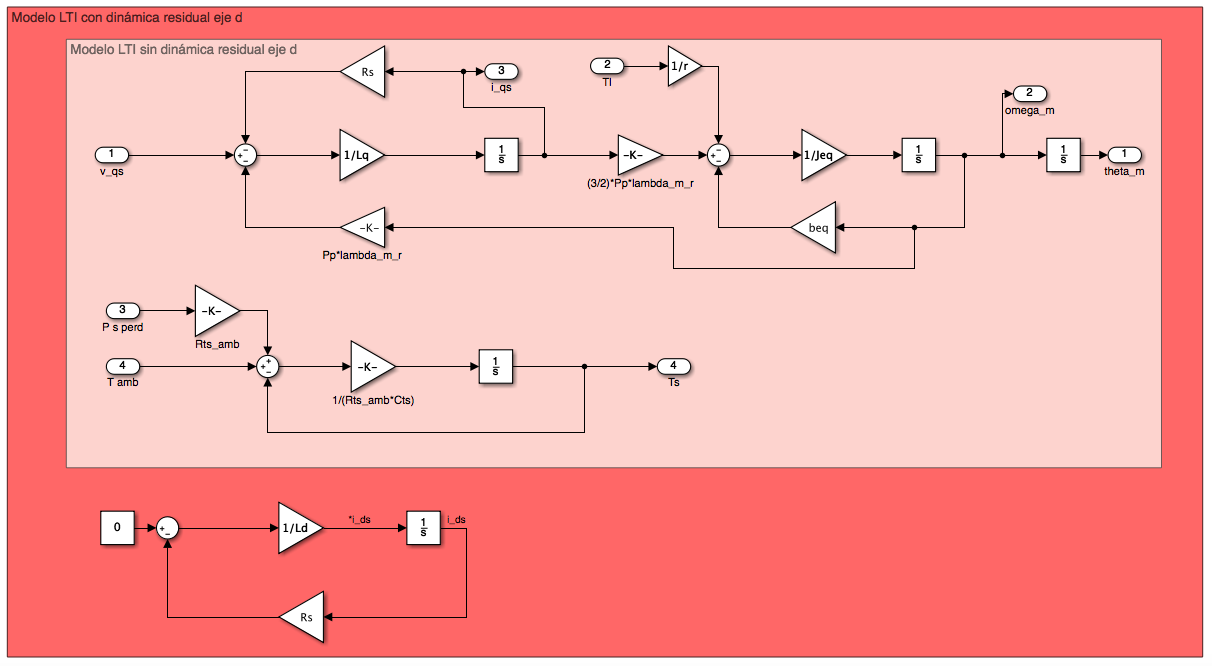
\includegraphics[width=0.5\textwidth]{DiagramabloquesLTI.png}
	\caption{\label{fig:diagLTI} Diagrama de bloques de estado del modelo simplificado lineal invariante (LTI) equivalente. Con dinámica residual (rojo) y sin dinámica residual (rosado) }
	\end{figure}
	
	\item\textbf{ Restricción o Ley de Control mínima}.
	Para lograr una $i^{r}_{ds}$ nula y asi obtener el modelo LTI desarrollado en el punto anterior debemos aplicar sobre el eje d la ley de control expresada por la ec. \ref{eq:2.1.2.d.1}.
	\begin{equation}
	v^{r}_{ds}(t)=-L_{q}*i^{r}_{qs}(t)*P_{p}*\omega_{m}(t)\ ; i^{r}_{ds}(t_{0})=0
	\label{eq:2.1.2.d.1}
	\end{equation}
	
	Esta restricción se obtiene al imponer la condición $i^{r}_{ds}\equiv 0$ en la ec.\ref{eq:}, lo que define una ecuación algebraica que representa una restricción sobre $v^{r}_{ds}(t)$. Asi $v^{r}_{ds}(t)$ deja de ser una variable manipulada. Como podemos ver se ha considerado que la condición inicial de $i^{r}_{ds}$ es nula, ya que si esta no lo fuera tendriamos una dinámica residual de la corriente $i^{r}_{ds}$ lo que provocaría que el modelo no sea lineal en los instantes iniciales, pero esto lo tocaremos en detalle más adelante. Por otro lado para implementar esta ley de control es necesario realimentar a nuestro controlador con las variables de estado $i^{q}_{ds}$ y $\omega_{m}$, y que este genere una consigna de tensiones de fase congruente con dicha restricción. Para ello en el controlador se implementa una transformación directa de Park para asi poder trabajar con las tensiones $v^{r}_{qd0s}$, ya que, de la planta sensamos $v_{abcs}$, asi generamos nuestras consignas de tensiones $v^{r}_{qd0s}$ y luego mediante una transformación inversa de Park obtenemos las tensiones de fase consignas $v_{abcs}$, capaces de reproducir dicha restricción, con las cuales generamos las consignas para alimentar al modulador de tensión, conmutado con modulación de ancho de pulso PWM. En este análisis el modulador de tensión se idealizado considerando solamente las componentes ideales de las ondas de tensión. Esta técnica se denomina \textbf{linealización por realimentación directa no lineal de estado parcial} y obtenemos asi el modelo \textbf{NL desacoplado con Ley de control NL}.\\
	 En el diagrama de bloques del modelo NL (figura \ref{})  podemos observar en rojo el desacoplamiento que esta restricción impone.\\
	  En la figura \ref{fig:diagrestriccionminima} se puede observar la implementación de esta ley de Control en color rojo dentro del controlador parcial.
	
	\begin{figure}[h!]
	\centering
	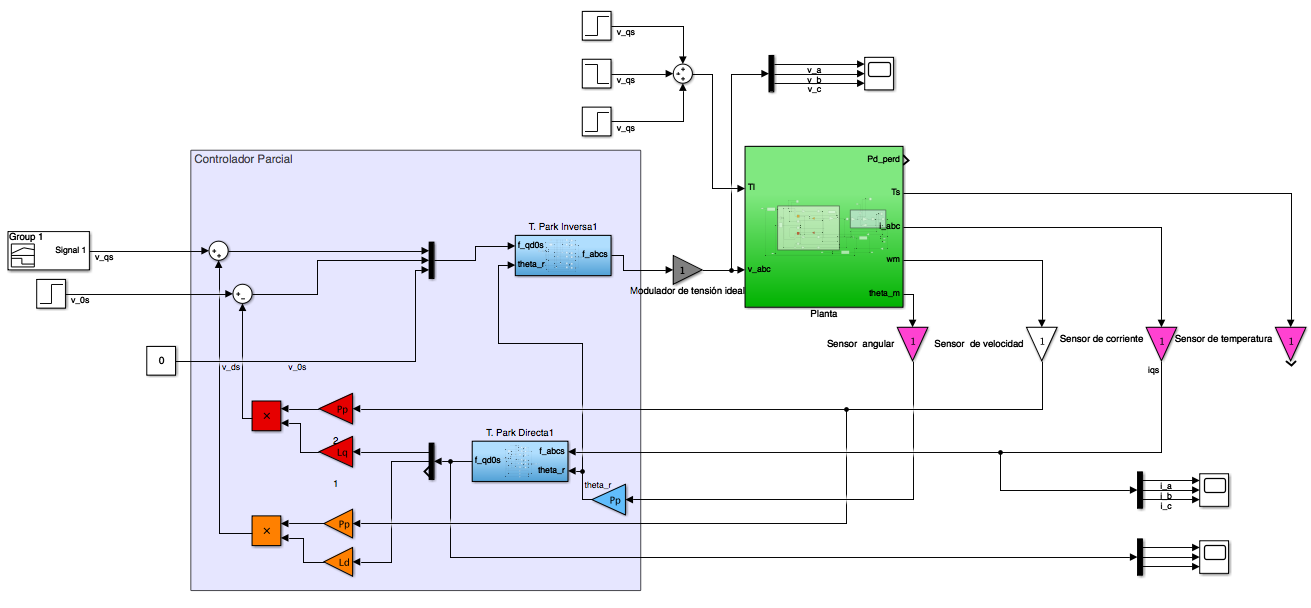
\includegraphics[width=\textwidth]{realimentacionNL.png}
	\caption{\label{fig:diagrestriccionminima} Impelementación controlador parcial con restricción mínima (rojo) y con restricción complementaria (naranja). Planta (verde), sensores(rojo), controlador parcial (cleste).}
	\end{figure}
	
	\item\textbf{Dinámica residual en el eje d}
	El modelo de la dinamica residual para para $i^{r}_{ds}$ esta dado por la ec.\ref{eq:2.1.2.e.1} y cuya ecuación de 				transeferencia esta dada por la ec.\ref{eq:2.1.2.e.2}.
	\begin{equation}
	\frac{di^{r}_{ds}}{dt}=\frac{R_{s}}{L_{d}}\ i^{r}_{ds}(t)
	\label{eq:2.1.2.e.1}
	\end{equation}
	\begin{equation}
	\frac{I^{r}_{ds}(s)}{E(s)}=\frac{1}{s+\frac{R_{s}}{L_{d}}}
	\label{eq:2.1.2.e.2}
	\end{equation}
	
	Vemos que la dinámica residual esta dada por una ecuación diferencial monótona descendiente con un cero en $s=-157.55$ si tomamos a $Rs$ constante e igual a 1.02. Por lo que podemos concluir que ante un estado inicial distinto de cero la corriente en el eje d va establecer rápidamente en cero.
	Si incorporamos esta dinámica residual a nuestro modelo LTI obtenemos:
	
	\begin{equation}
	X(t)=\begin{bmatrix}
	\theta_{m}(t)\\
	\omega_{m}(t) 
	\\ 
	i^{r}_{qs}
	\\
	i^{r}_{ds}
	\end{bmatrix}
	\label{eq:2.1.2.e.3}
	\end{equation}
	
	\begin{equation}
	\left\{\begin{matrix}
	\dot{X}(t)=\begin{bmatrix}
	0 & 1 &0 &0 \\ 
	0 & -\frac{b_{eq}}{J_{eq}} & \frac{3 P_{p} \lambda^{r'}_{m}}{2 J_{eq}} & 0 \\ 
	0  & \frac{- P_{p} \lambda^{r'}_{m}}{ L_{q}} & \frac{-R_{s}}{L_{q}}&0\\
	0&0&0&\frac{R_{s}}{L_{d}}
	\end{bmatrix} X(t) + \begin{bmatrix}
	0 &0 \\ 
	0 &\frac{-1}{J_{eq}} \\ 
	 \frac{1}{L_{q}}&0 \\
	 0&0
	\end{bmatrix} \begin{bmatrix}
	u(t)\\
	d(t) 
	
	\end{bmatrix} \ ; X(t_{0})=x_{0}\\ 
	y(t)=[1 \ \ 0 \ \ 0 \ \ 0 ] \ X(t)
	\end{matrix}\right.
	\label{eq:2.1.2.e.4}
	\end{equation}
	

	Donde vemos que ahora nuestro vector de estado (ec.\ref{eq:2.1.2.e.3}) tiene un estado más y las entradas son las definidas por las ec.\ref{eq:2.1.2.c.2} y ec.\ref{eq:2.1.2.c.3}. Como podemos ver ahora $i^{r}_{ds}$ puede ser distinta de cero, sin embargo no se ha considerado el acoplamiento residual Nl con el eje q (ec. \ref{eq:2.1.2.e.4}) y esto se debe a que como comentamos mas arriba la dinámica residual de este eje es monótona descendiente por lo que rápidamente $i^{r}_{ds}$ decae a cero, por lo que, en regimen forzado esta no va a tener influencia sobre el eje d.
	
	En la figura \ref{fig:diagLTI} se puede apreciar el modelo LTI considerando la dinámica residual del eje d (rojo).
	
	\begin{equation}
	v^{r*}_{qs}(t)=L_{d}. i^{r}_{ds}(t).P_{p}.\omega_{m}(t)
	\label{eq:2.1.2.e.4}
	\end{equation}
	
	   \item\textbf{Ley de Control complementaria mínima en el eje q}.
	    Para eliminar completamente este acoplamiento residual NL aún en régimen natural y obtener un modelo equivalente 				completamente lineal, independiente del estado inicial de $i^{r}_{ds}$ se debe realimentar al sistema con la ley de control 			dada por la ec.\ref{eq:2.1.2.e.4}. En la figura \ref{fig:diagrestriccionminima} se puede apreciar el controlador parcial con la implementación de esta restricción en color naranja, obteniendo asi el modelo \textbf{LTI equivalente aumentado} el cual aplica la ley de control mínima en el eje d y la ley de control complementaria en el eje q.\\
	     En el diagrama de bloques del modelo NL (figura \ref{})  podemos observar en naranja el desacoplamiento que esta restricción 		produce.\\
	\end{itemize}
	
	 \item Comparación del modelo dinámico LTI equivalente aumentado vs. el modelo dinámico global LPV forzando $I^{r}_{ds_{0}} =0$.
	 
\end{enumerate}


\subsubsection{Análisis de Estabilidad a lazo abierto para el modelo LTI equivalente aumentado}
\subsubsection{Análisis de Observabilidad completa de estado para el modelo LTI equivalente aumentado}
\subsubsection{Análisis de Controlabilidad completa de estado para el modelo LTI equivalente aumentado}
\subsubsection{Simulación dinámica en DT, comparando el modelo NL completo desacoplado con Ley de control
NL vs LTI equivalente aumentado}


\subsection{Diseño, Análisis y Simulación con CONTROLADOR de Movimiento en Cascada con Modulador de Torque equivalente (Control Vectorial)}
\subsubsection{Modulador de Torque equivalente (Controlador interno vectorial de corriente/torque)}
\subsubsection{Controlador externo de movimientos: posición/velocidad }
\subsubsection{IncorporaciónydiseñodeObservadordeEstadodeordenreducidosóloparalapartemecánica de este controlador}
\subsubsection{Simulación en tiempo continuo con modelo completo NL}
\subsubsection{Verificacióndedesempeñoy/omejoras}

\section{Conclusiones}

\section{Referencias}

\end{document}